\chapter{Grundlagen}

Ziel dieser Arbeit ist die Ermittlung optimierter Gebäudeenergiesysteme für den deutschen Wohngebäudebestand.
Hierzu wurde in Kapitel \ref{sec:Sektion 21} der Bestand analysiert, um auf dieser Untersuchung aufbauend die nationale Wohngebäudesituation in einigen wenigen, repräsentativen Klassen abzubilden. 
Des Weiteren wurde in \ref{sec:Sektion 22} die historische Entwicklung der deutschen Dämmstandards betrachtet. Daraus wurden Zeiträume der Baualtersklassen mit ähnlichen Wärmeübergangskoeffizienten der Gebäudehülle zusammengefasst. 
Zuletzt stellt Kapitel \ref{sec:Sektion 23} die Grundlagen der mathematischen Optimierung sowie das im Rahmen dieser Arbeit erweiterte Optimierungsprogramm vor. 

Die Gebäudeklassen sollen für die Bestimmung der Gebäudeenergiesysteme mit dem Optimierungsprogramm benutzt werden. 
Hieraus soll ein Vergleich zwischen Emissionsoptimum sowie Kostenoptimum gewonnen werden.

%Gebäudeenergiesysteme erklären?
%Was hat das überhaupt mit Grundlagen zu tuen, was ich da schreibe?
%Nehm ich in der Einleitung des Kapitels hier zuviel vorweg?
%Ist es okay, hier den Vergleich zu erwähnen? Evl. umschreiben
%Letzter Satz beschissen


\section{Deutscher Wohngebäudebestand}
\label{sec:Sektion 21}

Zunächst wurde der Wohngebäudebestand hinsichtlich Alter und Größe ausgewertet.
Als Daten wurden die Statistiken des Zensus2011, einer nationalen statistischen Erhebung von privaten Haushalten, betrachtet. 
Besagte Statistiken wurden in verschiedenen wissenschaftlichen Untersuchungen des Institut für Wohnen und Umwelt GmbH (IWU) ausgewertet und evaluiert.
Weiterhin wurde für die gebäudetypischen Kennwerte die Typgebäude des europaweiten TABULA Projekts berücksichtigt.

Nach den 2011 veröffentlichten Zensus Daten besteht der deutsche Wohngebäudebestand aus rund 18.368.000 Gebäuden mit 39.432.000 Wohnungen \cite{.2015}.
Wie in Abbildung \ref{fig: Abbildung211} zu erkennen ist, prägt den deutschen Wohngebäudebestand einen Boom in der Nachkriegszeit. 
So wurden in den Jahren von 1949 bis 1978 etwa 7,2 Millionen Häuser errichtet. Diese Klasse alleine macht \mbox{38 \%} der deutschen Wohngebäude aus. 
Mit ca. 2,7 Millionen Gebäuden und einem Anteil von etwa \mbox{14 \%} bilden die vor 1919 fertiggestellten Wohnobjekte den zweitgrößten Anteil, sowie die Häuser mit Baualter zwischen 1919 und 1948 mit knapp \mbox{12 \%} die drittgrößte Gruppe.
Folglich sind knapp zwei Drittel der deutschen Wohngebäude vor 1978 erbaut worden.

Eine weitere relevante Klasse beschreiben mit fast \mbox{10 \%} die von 1979 bis 1986 geschaffenen Wohnbauten. 
Zusammen mit den drei Klassen \mbox{1987 - 1990,} \mbox{1991 - 1995} und \mbox{1996 - 2000} werden  durch diese vier Gruppen mehr als ein Viertel des Wohngebäudebestandes in Deutschland abgebildet.

Im Gegensatz zu den zuvor genannten Gruppen stellen die nach der Jahrtausendwende konstruierten Häuser mit unter \mbox{10 \%} und nur 1,6 Millionen Häusern einen relativ kleinen Anteil des nationalen Bestandes dar. 

\begin{figure}[H]
	\centering
		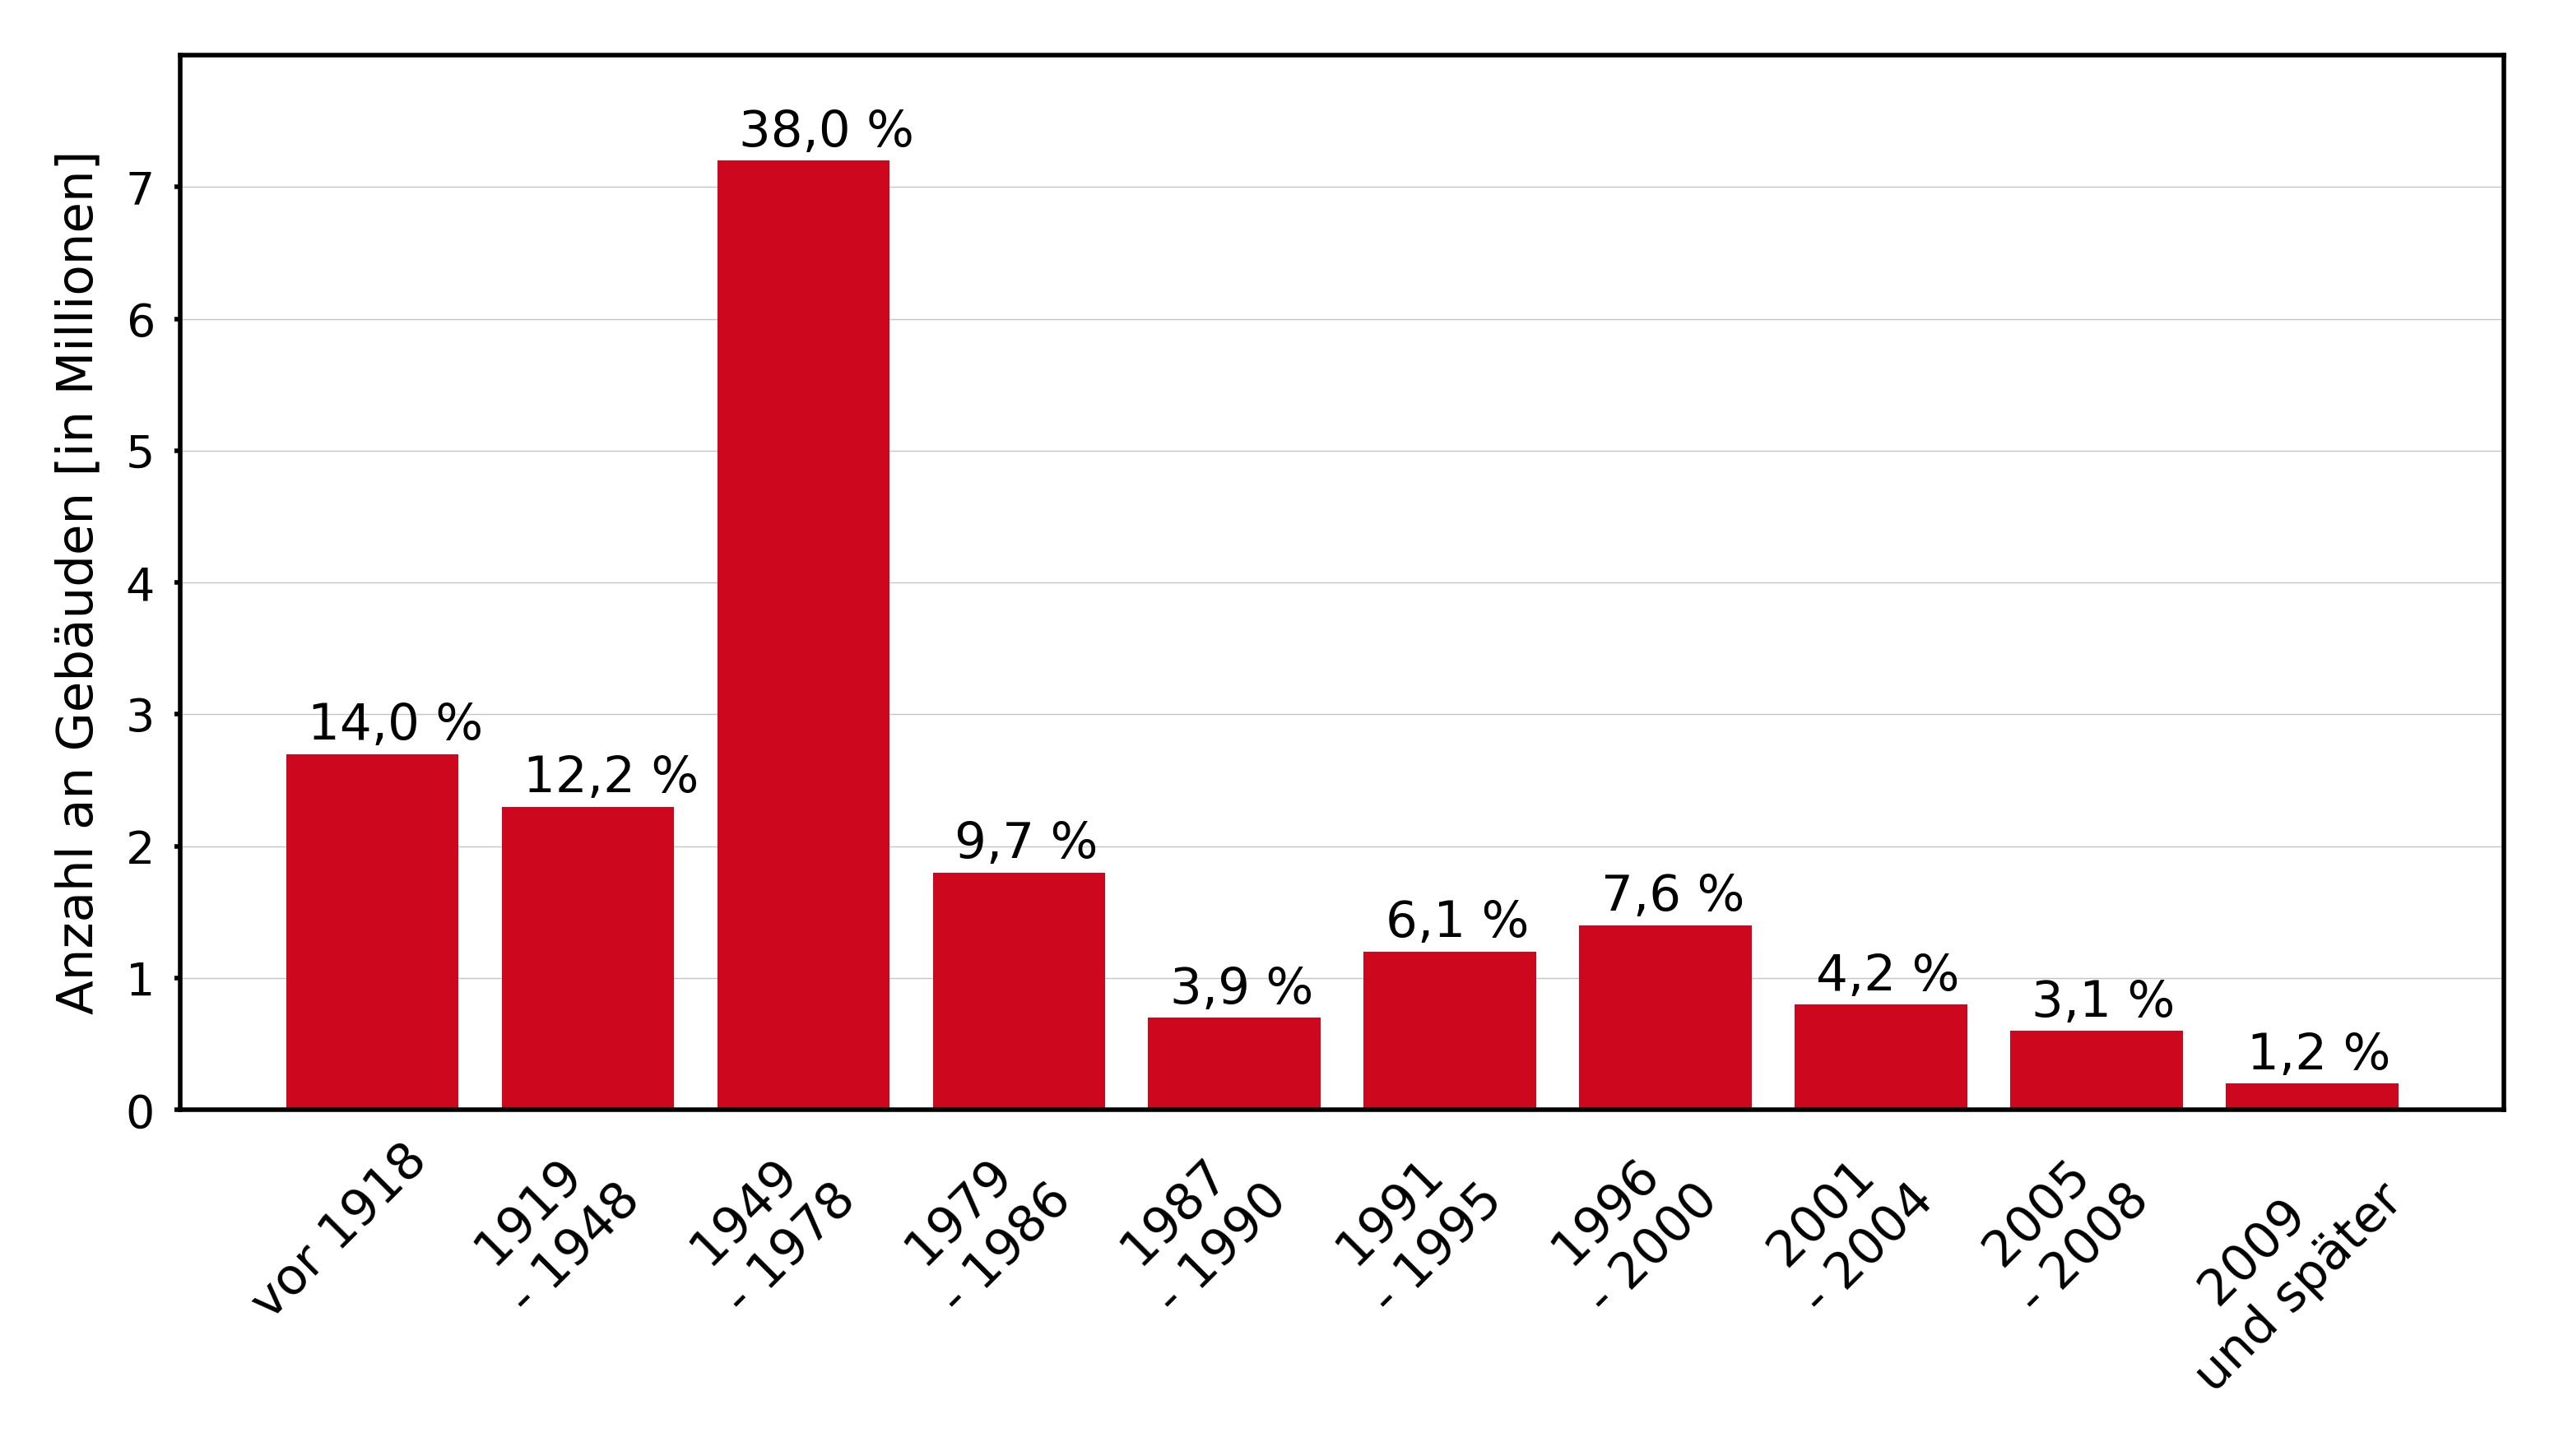
\includegraphics{Pictures/GebaeudeAlterDiagramm.jpg}
	\caption{errichtete Wohngebäude nach Mikrozensus-Klassen  	\cite{StatistischeAmterdesBundesundderLander.2014}}
	\label{fig: Abbildung211} 
\end{figure}

Es sei noch zu erwähnen, dass in dieser Betrachtung den Mikrozensus-Klassen gefolgt wurde. 
Diese sind explizit keine gleich langen Zeitintervalle, sondern \glqq orientieren sich an historischen Einschnitten, den Zeitpunkten statistischer Erhebungen und den Veränderungen der wärmetechnisch relevanten Bauvorschriften\grqq \cite{.2015}. 
So beschreibt beispielsweise das relativ kurze Zeitintervall von 1979 bis 1983 den Zeitraum zwischen erster und zweiter Wärmeschutzverordnung, auf welche in Kapitel \ref{sec:Sektion 22} noch näher eingegangen wird.

Eine weitere Unterteilung des Wohngebäudebestandes erhält man bei der Betrachtung der Anzahl an Wohneinheiten im Gebäude. 
Hierbei setzt sich der Bestand zu zwei Dritteln aus Wohngebäuden mit nur einer Wohnung zusammen. 
Weitere \mbox{17 \%} bilden Gebäude mit zwei Wohnungen und die Klasse der Gebäude mit \mbox{3 - 6 Wohnungen} stellen \mbox{12 \%.} 
Die größeren Gebäude mit \mbox{7 - 12 Wohnungen} sowie mit 13 und mehr Wohnungen sind anteilig am Gebäudebestand mit jeweils \mbox{5 \%} und \mbox{1 \%} relativ kleine Gruppen. 
Allerdings gelten letztere nur bei einer Gebäudebetrachtung als weniger relevant, da sie bei einer Anschauung der Wohneinheiten logischerweise mit größeren Faktoren eingehen. \cite{StatistischeAmterdesBundesundderLander.2014b}

In Abbildung \ref{fig: Abbildung212} sind die Anzahl der Wohneinheiten für die drei Baualter-Klassen älter als 1978, \mbox{1979 - 1994} und \mbox{1995 - 2009} sowie deren Anteil an allen Wohneinheiten bis Baujahr 2009 des Gebäudebestandes dargestellt. 
In Anlehnung an den vorherigen Abschnitt werden Gebäude mit bis zu 2 Wohnungen als Einfamilienhäuser zusammengefasst und nach der Englischen Bezeichnung \glqq single family home\grqq mit SFH abgekürzt. 
Wohngebäude mit 3 oder mehr Wohnungen werden als Mehrfamilienhäuser mit der Abkürzung MFH für \glqq multy family home\grqq gebündelt. 

Auffallend ist wiederum der enorme Anteil der Gebäude mit Baualter älter als 1978. 
Hier zählen die Mehrfamilienhäusern mit 14,8 Millionen Wohnungen und einem Anteil aller bis 2009 errichteten Wohneinheiten von \mbox{38 \%} zur größten Gruppe. 
Mit 12,5 Millionen Wohnungen und einem Anteil von 32\,\% entfällt die zweitgrößte Klasse auf die Einfamilienhäuser mit Baujahr älter 1978.
Ähnlich wie zuvor bei der Gebäudebetrachtung sind somit auch mehr als zwei Drittel aller Wohnungen vor 1978 erbaut worden.


\begin{figure}[H]
	\centering
		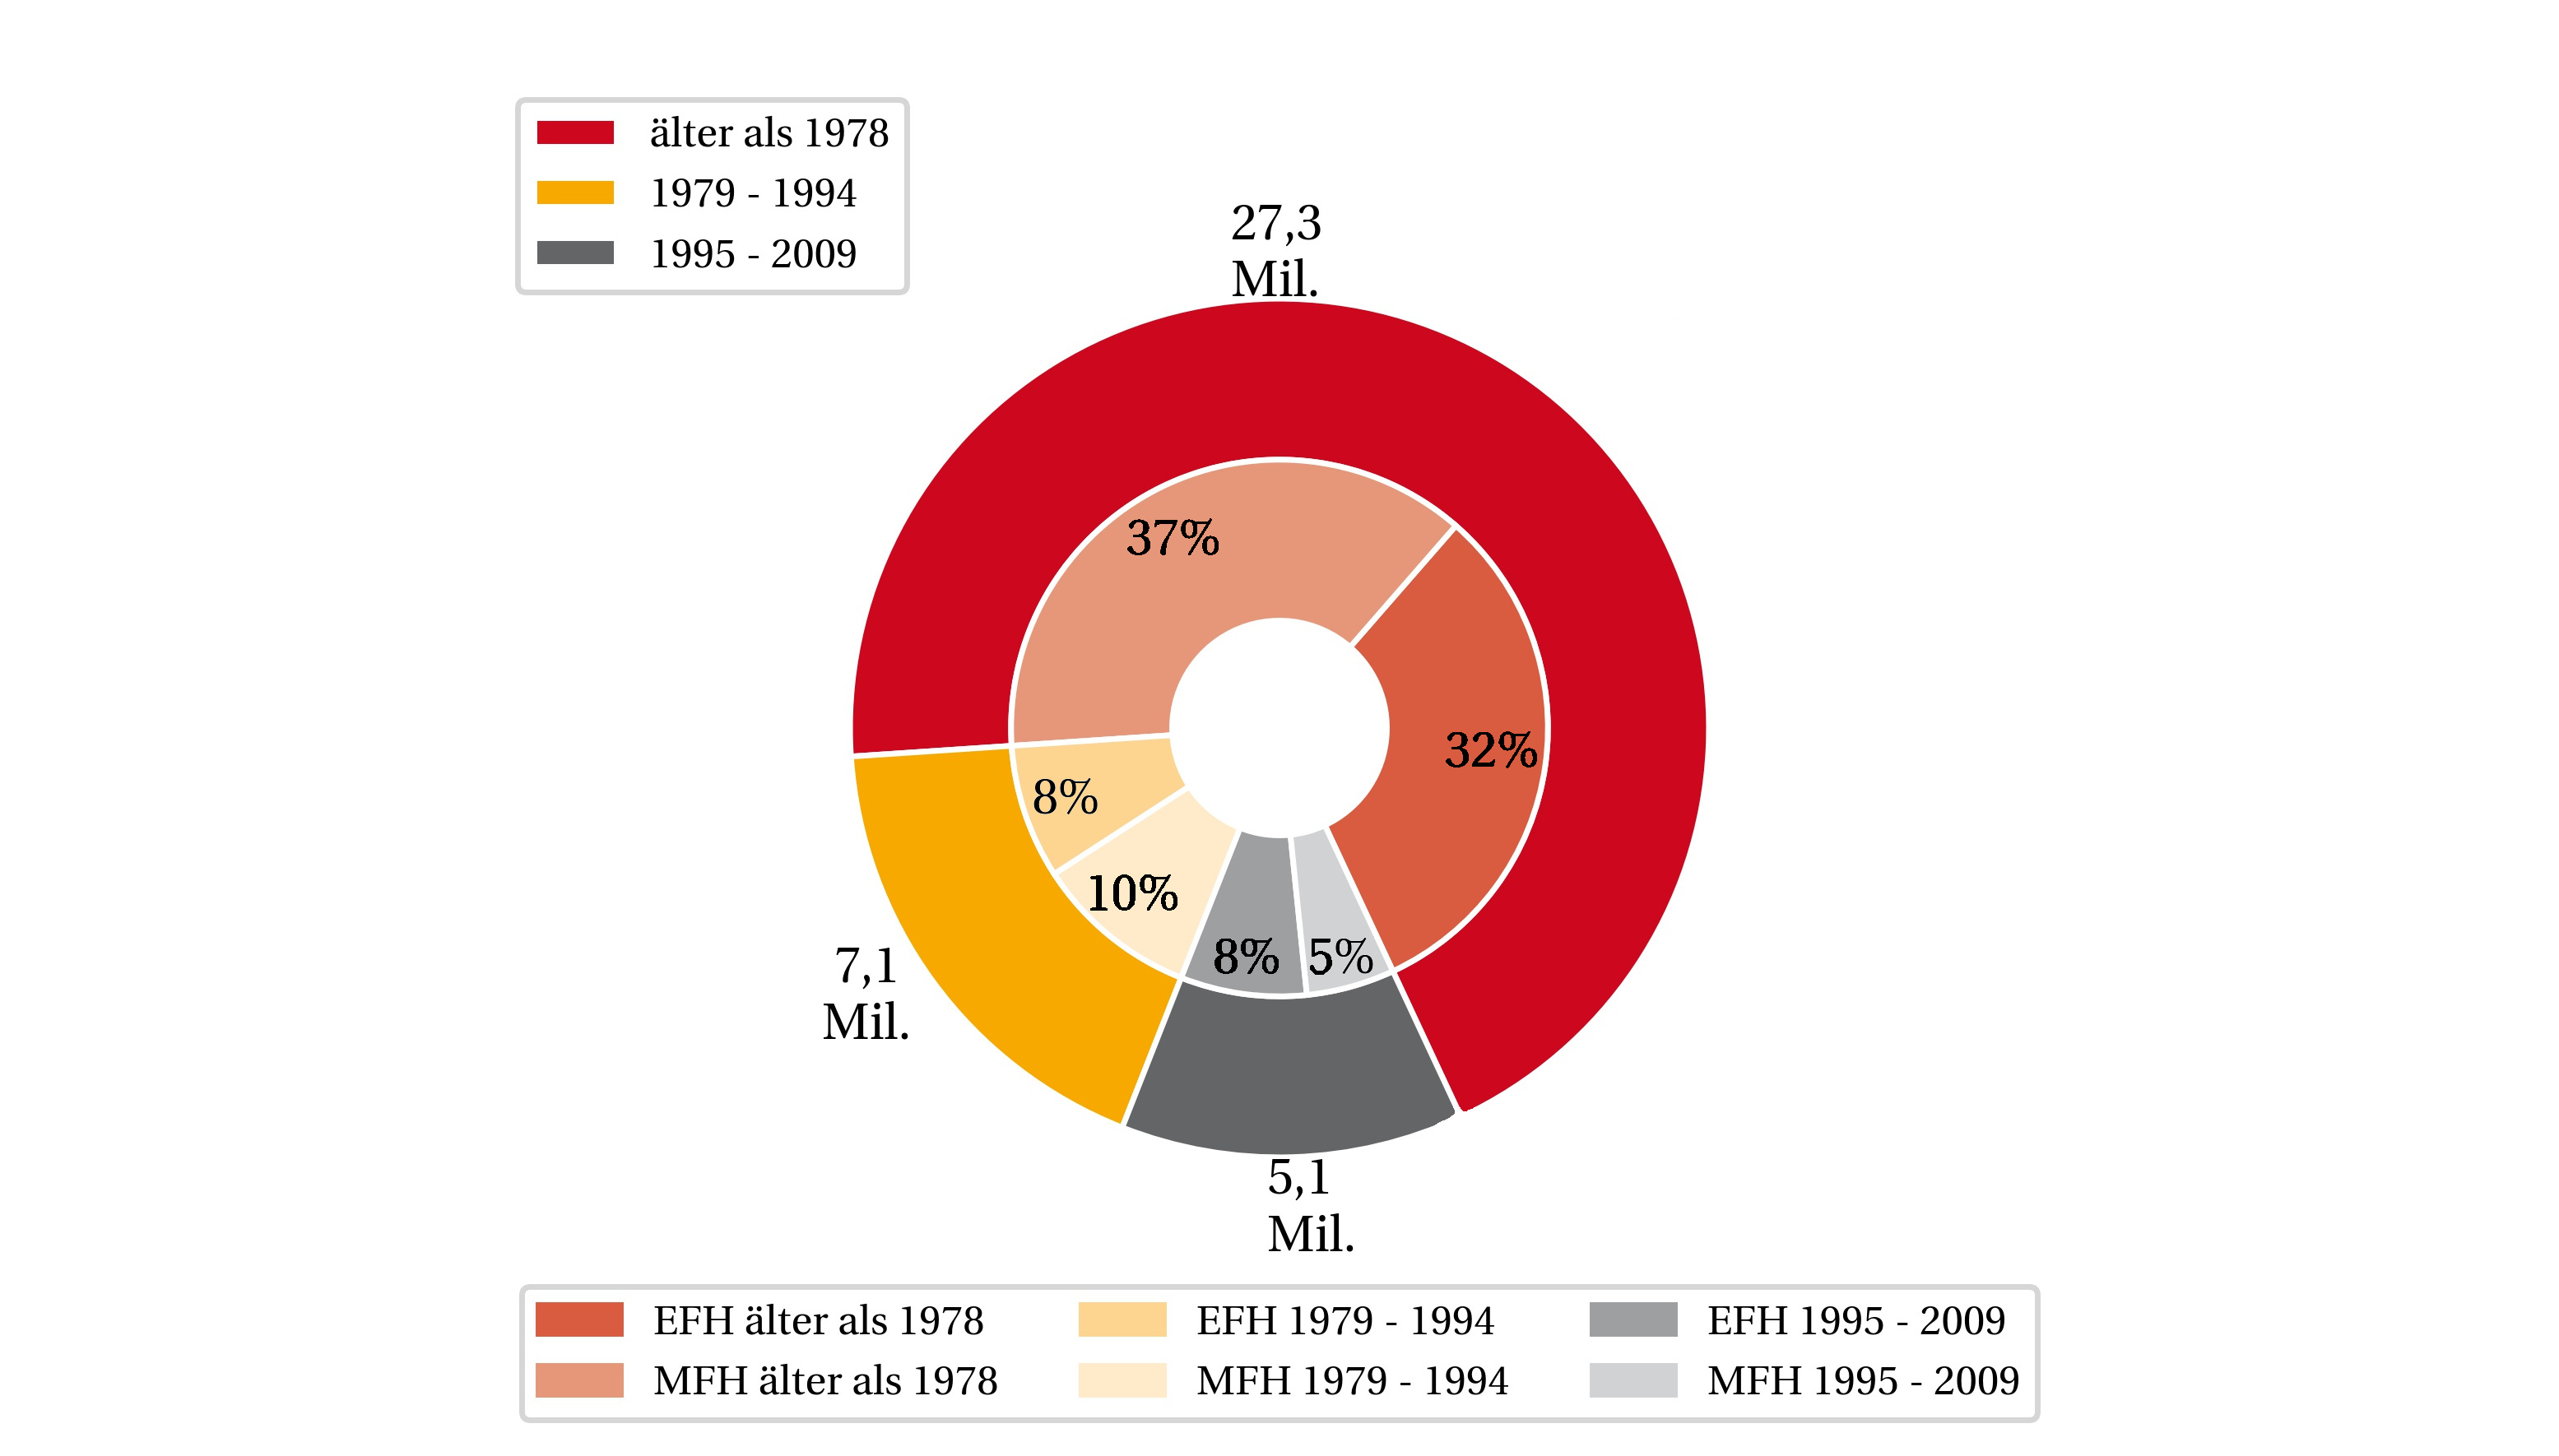
\includegraphics{Pictures/GebaeudeGroesse.jpg}
	\caption{Anzahl an Wohneinheiten bei Einfamilienhäuser (SFH) und Mehrfamilienhäuser (MFH) \cite{StatistischeAmterdesBundesundderLander.2014b}}
	\label{fig: Abbildung212} 
\end{figure}



%Wohnobjekte?
%Zensus näher erläutern?
%Auf jeden Fall TABULA und Typgebäude näher beschreiben.

\section{Historische Entwicklung der Dämmstandards}
\label{sec:Sektion 22}

Nachdem im vorherigen Kapitel der Gebäudebestand nach Alter und Größe beschrieben wurde, werden nun die zu den jeweiligen Gebäudealtern und -größen zugehörigen Dämmstandards vorgestellt. 
Da die Dämmung eines Gebäudes dessen Wärmeverluste und folglich dessen Endenergieverbrauch beeinflusst, stellt diese ein wichtiges Charakteristikum zur Klassifizierung des Bestandes dar.

%Dämmung kurz allgemein erklären, um den letzten Satz zu begründen + Einstieg für Gründerzeit

bis 1918: period of promoterism ("Gründerzeit"), rapid expansion of the cities and growing industrialisation; standardisation of construction principles; differ-ent regional manifestations

1919 - 1948: increasing industrialised production of building materials; use of cost effi-cient material-saving constructions; standardisation on national level

1949 - 1957: simple building techniques of the post-war period; often use of debris mate-rials; further development of construction standards (introduction of DIN 4108 – "Wärmeschutz im Hochbau" in 1952); introduction of social housing principles

1958 - 1968: requirements on thermal insulation in force (DIN 4108 – "Wärmeschutz im Hochbau"); further industrialisation of building construction; development of panel buildings (GDR: "Plattenbauten")

1969 - 1978: new industrial building techniques (sandwich elements); also introduction of pre-fabricated single family houses (lightweight constructions "Fertighaus"); thermal insulation becomes more relevant in consequence of the first oil crisis

1979 - 1983: 1st thermal protection ordinance (1. Wärmeschutzverordnung)

1984 - 1994: 2nd thermal protection ordinance (2. Wärmeschutzverordnung); GDR: further improved insulation ("Rationalisierungsstufe III")
market introduction of low energy houses, supported by regional grant pro-grammes

1995 - 2001: 3rd thermal protection ordinance (3. Wärmeschutzverordnung); considera-tion of a bonus in the tax in case of realisation of a low energy house

2002 - 2009: energy saving ordinance ("EnEV 2002"), considering building and heat supply system; KfW grant programmes ("KFW-Energiesparhaus 60 and 40”, Passive Houses)

2010 ... : new requirements of energy saving ordinance ("EnEV 2009") on the level of low energy buildings
new KfW grant programme regulations ("KFW-Effizienzhaus 70, 55 and 40”, Passive Houses)

\begin{figure}[H]
	\centering
		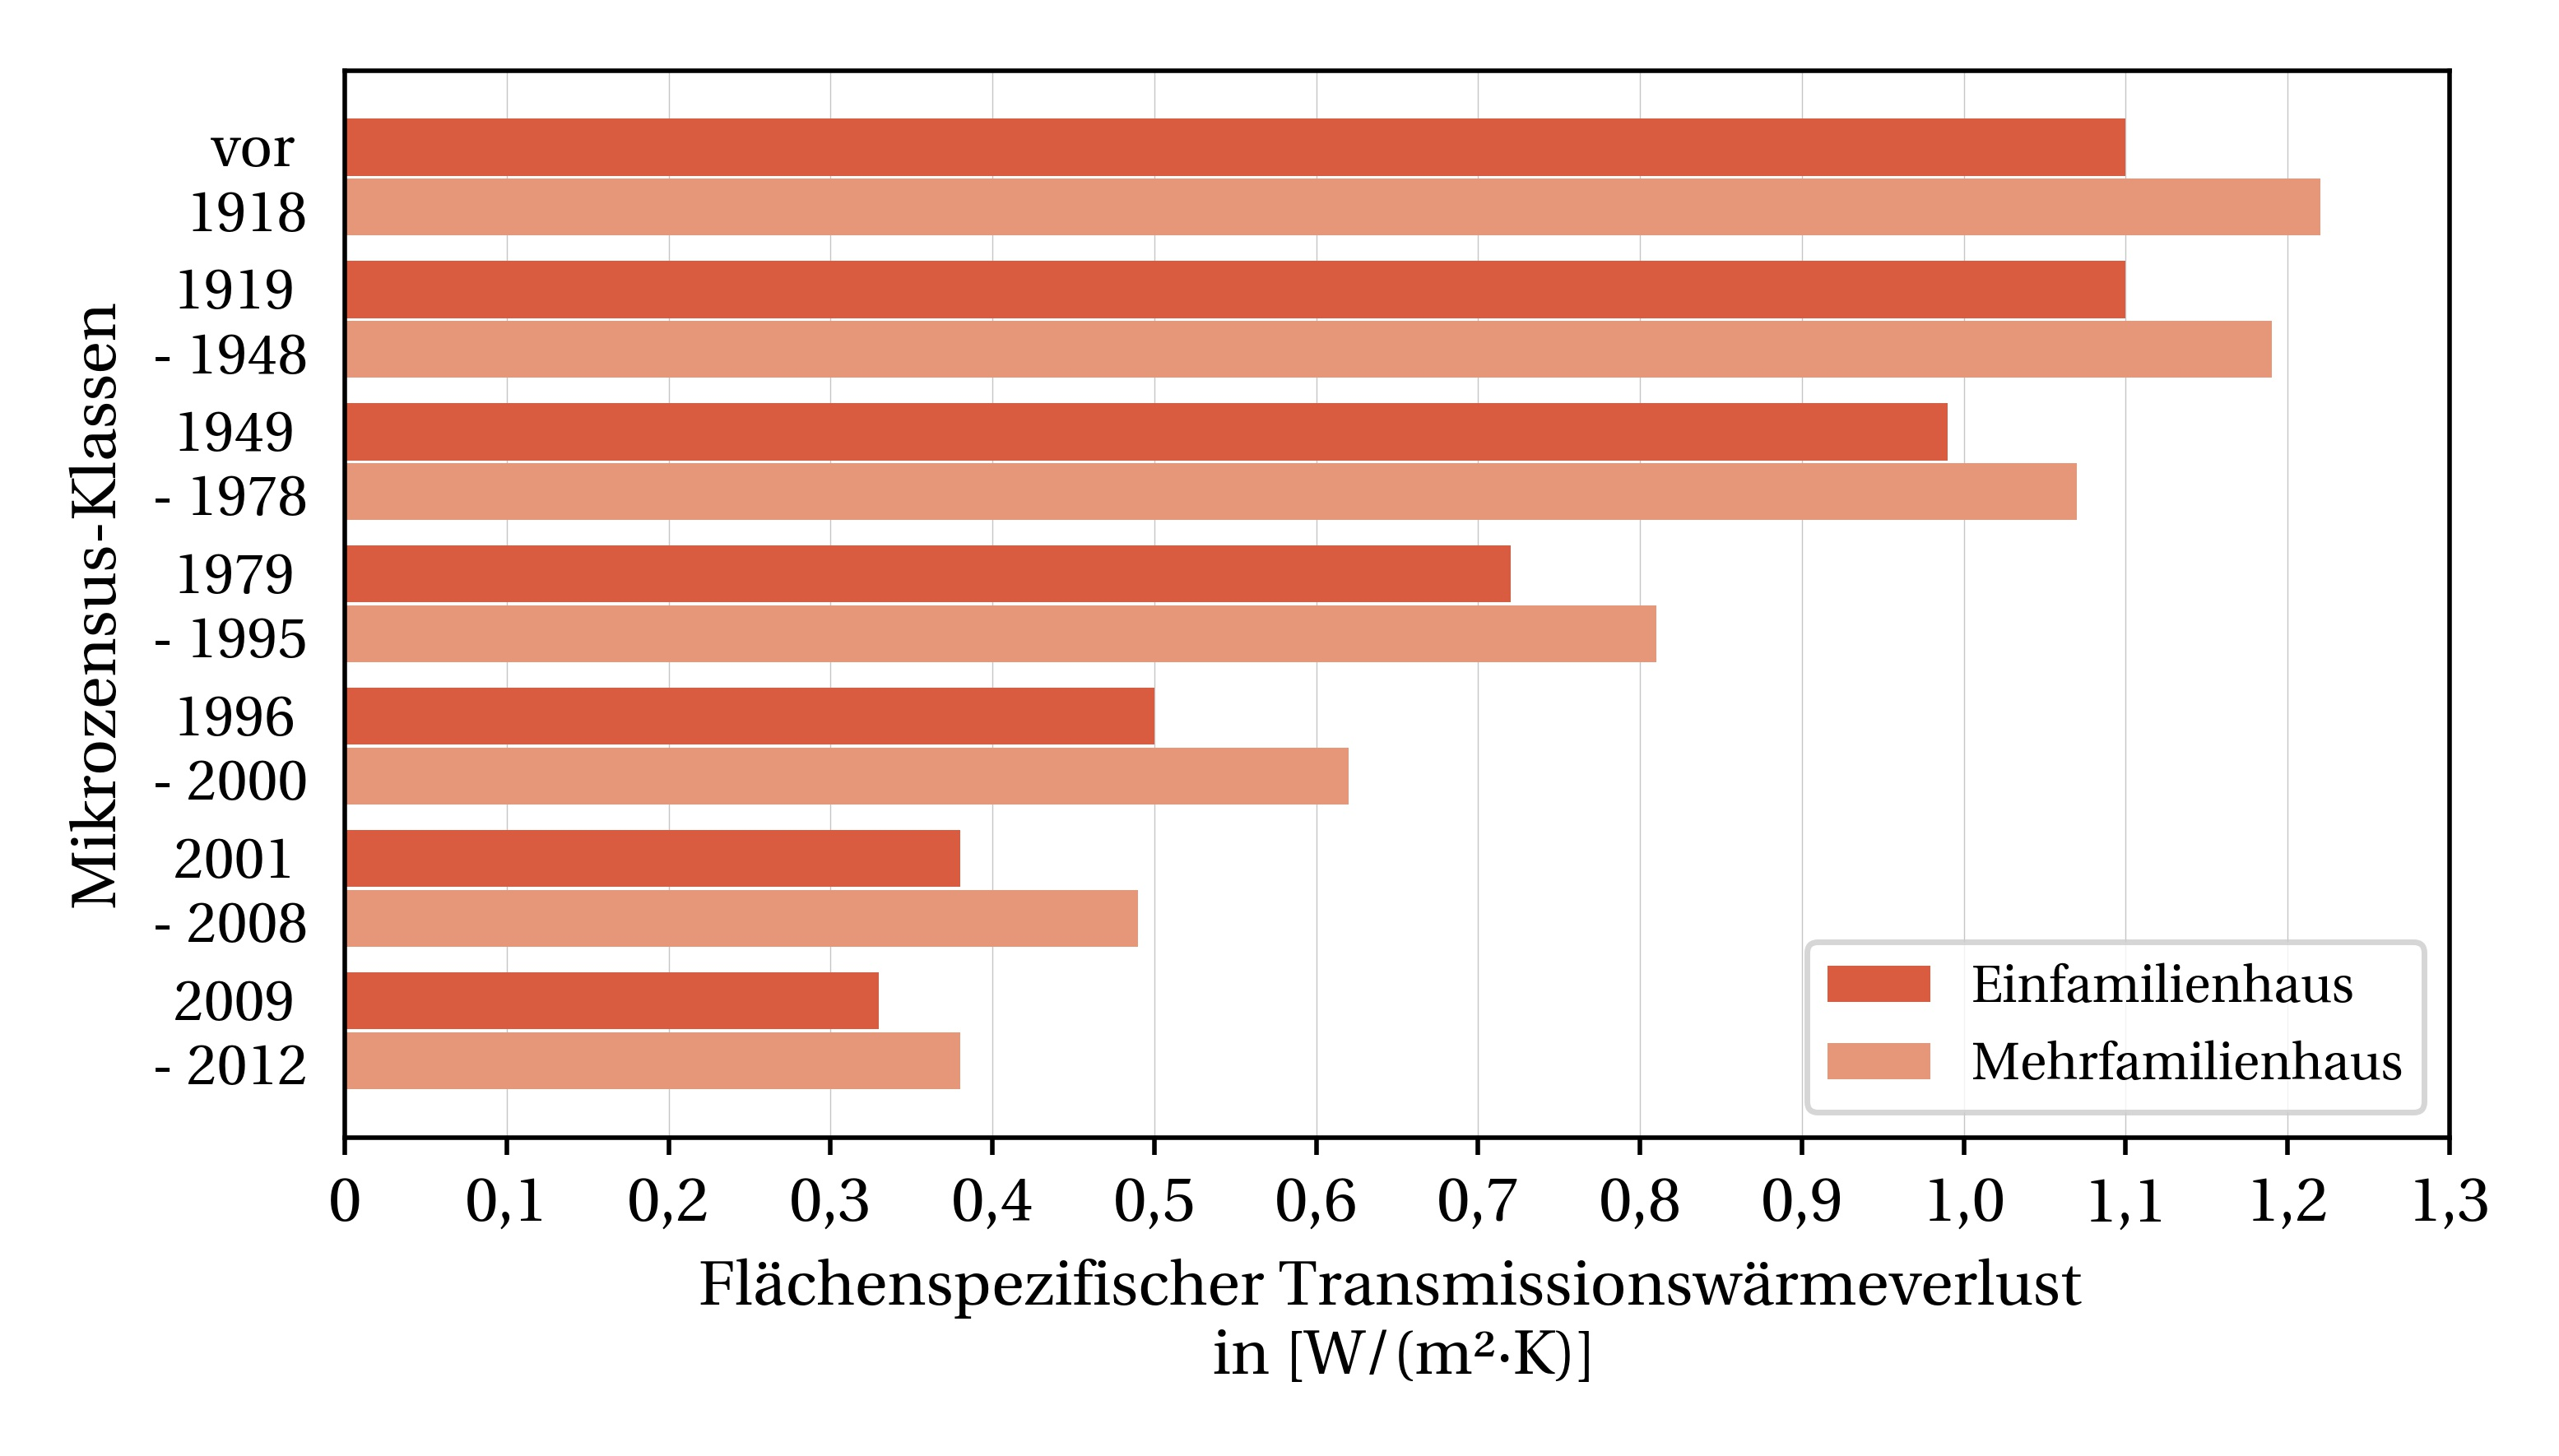
\includegraphics{Pictures/TransmissionswaermekoeffizientBaujahr.jpg}
	\caption{tba}
	\label{fig: Abbildung221} 
\end{figure}

\section{Sanierungsstand des deutschen Wohngebäudebestandes}
\label{sec:Sektion 23}


\section{Optimierungsmodell}
\label{sec:Sektion 24}



